\documentclass[11pt,a4paper]{article}
\usepackage{acl2015}
\usepackage{url}
\usepackage{latexsym}
\usepackage{graphicx}
% \usepackage{indentfirst}


\title{Asignatura Text Mining II\\
M\'aster/Diploma Big Data Analytics}

\author{Pedro Henrique Mano Figueiredo Fernandes \\
  {\tt pedromorfeu@gmail.com} \\}

\date{\today}

\begin{document}
\maketitle
\begin{abstract}

  La aproximaci\'on al problema de {\em Text Mining} para {\em Author Profiling} ha tenido como base la t\'ecnica conocida por {\em bag of words}. Esta t\'ecnica consiste en el aprendizaje del vocabul\'ario de un conjunto de documentos, a trav\'es del que se construye una representaci\'on de los datos en forma de matriz num\'erica, adecuada para aplicar {\em machine learning}. A la matriz de vocabulario se han a\~nadido otras caracter\'isticas, como contadores de polaridad de sentimientos y determinadas estad\'isticas del texto de los documentos. El {\em metadata} de los tweets se ha usado tambi\'en para reforzar las caracter\'isticas de la matriz.
  El modelo usado para el aprendizaje del vocabul\'ario se basa en contadores de palabras, calculando un coeficiente de tipo TF-IDF. Se ha configurado el modelo con un m\'aximo de 2000 caracter\'isticas, que se traduce en el c\'alculo de las 2000 palabras más significativas en el corpus de entrenamiento. Para la divisi\'on de los documentos en trozos ({\em tokens}) se han aplicado {\em tokenizers} especializados en texto de Twitter.
  Una vez constru\'ida la matriz con todas las caracter\'isticas, se ha elegido un clasificador de tipo {\em Random Forest} para entrenar un modelo matem\'atico. Este clasificador es de tipo {\em ensemble}, aplicando varias iteraciones de predicci\'on sobre conjuntos aleat\'orios de los datos, lo que garantiza una mejor robustez y generalizaci\'on del modelo.

\end{abstract}


\section{Introducci\'on}

  La exploraci\'on de datos de lenguage natural permite descubrir caracter\'isticas de los autores basadas en sus patrones de escrita. El objectivo de este ejerc\'icio es explorar la informaci\'on de un dataset constitu\'ido por {\em tweets} de varios usuarios de distintos pa\'ises de habla hisp\'anica, con el intuito de crear un modelo clasificador de perfiles de sexo y pa\'is.

  Determinados patrones de escrita pueden mostrar ind\'icios de perfiles. Algunos estudios indican que los hombres tienen tendencia a usar m\'as determinantes y adjectivos que las mujeres; y las mujeres suelen usar m\'as pronombres y la negaci\'on. En general, las mujeres tienen tendencia a demostrar m\'as carga emocional en sus frases que los hombres. M\'etricas como el tama\~no de las frases pueden eventualmente ser significativas tambi\'en. Adem\'as, hay que tener en cuenta los usuarios corporativos, cuya escrita ser\'a diferente de la de otros perfiles, probablemente m\'as formal.

  De la misma forma, los perfiles de pa\'ises obedecen a patrones de escrita, con elementos significativos como el uso de modismos y otras variaciones lengu\'isticas. 

  El corpus de texto se usa para aprender el vocabul\'ario significativo y luego aplicar t\'ecnicas de {\em machine learning}, que se encargar\'an de encontrar patrones y correlaciones para generar un modelo matem\'tico. Los datos sirven como mat\'eria prima, a la que se aplican herramientas para crear nuevo conocimiento.


\section{Dataset}

  El dataset de este ejerc\'icio est\'a constitu\'ido por cientos de {\em tweets} de usuarios de 7 pa\'ises de habla hisp\'anica. Cada pa\'is tiene {\em tweets} de 650 usuarios y cada usuario tiene entre 600 y 1000 {\em tweets}. 

  El conjunto de entrenamiento cuenta con datos de 2730 usuarios previamente clasificados en sexo y pa\'is. En total hay 2.616.338 tweets, que constituye el corpus para calcular el vocabulario. El conjunto de test tiene 1820 usuarios y respectiva clasificaci\'on, con un total de tweets de 1.741.060. El volumen de datos es bastante grande y de c\'omputo exigente: en una m\'aquina con 4GB de RAM y un procesador i3, el c\'alculo del vocabulario para solamente 2000 palabras tarda m\'as de 10 minutos.

  Se ha realizado un breve an\'alisis estad\'istico sobre la matriz de {\em bag of words} con R, cuyos resultados se presentan a continuaci\'on. El gr\'afico siguiente representa las palabras y s\'imbolos con mayor coeficiente TF-IDF. Se verifica que las palabras m\'as significativas son tambi\'en las m\'as usuales - este dato ser\'a relevante en el desarrollo del estudio propuesto.
  
  \begin{figure}[ht!]
    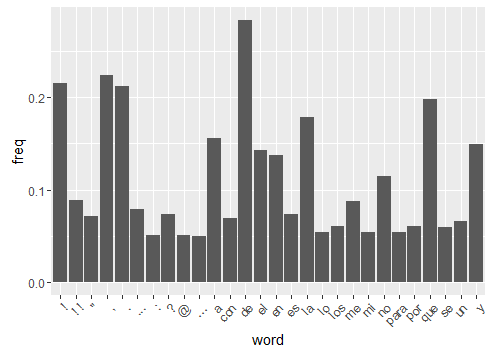
\includegraphics[width=\linewidth]{most_used_words.png}
    \caption{Palabras con mayor coeficiente TD-IDF.}
    \label{fig:most_used_words}
  \end{figure}
    
  En un breve an\'alisis de sentimientos (positivo y negativo), se puede ver que la media es ligeramente superior en las mujeres.
  
  \begin{figure}[ht!]
    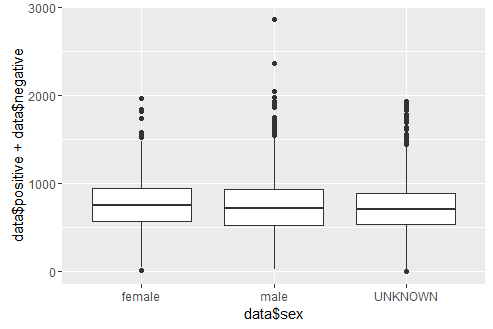
\includegraphics[width=\linewidth]{sentiment.png}
    \caption{Sentimiento.}
    \label{fig:sentiment}
  \end{figure}
  
  El tama\~no medio de frases muestra que los hombres escriben frases m\'as largas; interesante que el tama\~no medio de las frases de mujeres y desconocido ({\em UNKNOWN}) es parecido:

  \begin{figure}[ht!]
    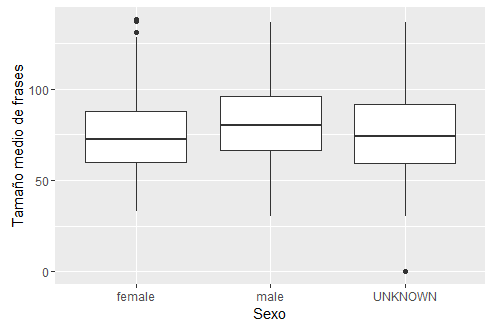
\includegraphics[width=\linewidth]{sentence_mean.png}
    \caption{Tama\~no medio de frases.}
    \label{fig:sentence_mean}
  \end{figure}
  
  El {\em metadata} de los tweets puede contener datos significativos. Se han usado sobre todo los colores usados en el perfil de {\em Twitter}. Por ejemplo, en el elemento {\tt profile\_sidebar\_fill\_color}, se pueden identificar algunos patrones:
   
  \begin{figure}[ht!]
    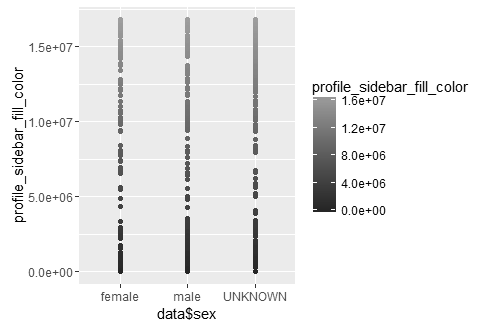
\includegraphics[width=\linewidth]{profile_colors.png}
    \caption{Colores del perfil de Twitter.}
    \label{fig:profile_colors}
  \end{figure}
  

\section{Propuesta del alumno}

  La estrat\'egia para generar el corpus de texto ha sido la siguiente: el texto de los {\em tweets} de cada usuario se ha acumulado en un documento \'unico. Cada documento se guarda en memoria, en una lista de documentos, uno por cada usuario. Esta lista es la que se pasa al {\em vectorizer} para aprender el vocabulario y calcular las frecuencias TF-IDF.

  La t\'ecnica {\em bag of words} ha dado un {\em baseline} para acercar el problema. Esta t\'ecnica se basa sencillamente en contadores de palabras, en su concepto. Sin embargo, se puede customizar la forma de contar (acumulador, cuoficiente, bin\'ario), la forma de separar los componentes del texto, el n\'umero m\'aximo de palabras del vocabulario o conjuntos de varias palabras. Las decisiones de configuraci\'on se describen a continuaci\'on.

  Se ha usado un {\em tokenizer} especializado en texto de {\em tweets} ({\tt TweetTokenizer}, del paquete {\em NLTK}), que ofrece opciones de ignorar referencias a otros usuarios y reducir las repeticiones de texto. Se ha usado tambi\'en la opci\'on de tratamiento {\em case-sensititve}, por poder ser significativo en la distinci\'on de g\'enero.

  La transformaci\'on de los datos en caracter\'isticas num\'ericas adecuadas para {\em machine learning} es un \'area conocido por {\em feature extraction}; en el caso de {\em bag of words} el proceso es de vectorizaci\'on, generando un vector de caracter\'isticas. Para esta tarea se ha usado la clase {\tt TfidfVectorizer} de {\em scikit-learn}, que implementa la separaci\'on en {\em tokens} y el c\'alculo de frecuencias, así como la normalizaci\'on y atribuci\'on de pesos de importancia a las palabras. Se ha configurado el modelo para generar una matriz de caracter\'isticas de cuoficientes TF-IDF.

  El aprendizaje del vocabulario es una tarea intensiva para CPU y memoria, directamente proporcional al numero de caracter\'isticas/palabras del vector generado. Se ha configurado el modelo para un m\'aximo de 2000 palabras, que presentaba rendimiento y resultados aceptables. Sin embargo, se han realizado pruebas y se ha verificado que los resultados de predicci\'on son mejores con mayor numero de caracter\'isticas, a coste de mayor tiempo de ejecuci\'on. Otra configuraci\'on importante es el rango de {\em ngrams}, que son conjuntos de palabras consecutivas. Se ha aplicado el rango de 1 a 2 palabras, con lo que se han mejorado los resultados.

  Determinadas palabras son muy comunes y aparentemente aportan poco significado, como es el caso de art\'iculos y preposiciones, como ``de``, ``la``, ``para``. Estas palabras se llaman {\em stop words}. La clase {\tt TfidfVectorizer} ofrece la posibilidad de usar una lista de {\em stop words} y el paquete {\em NLTK} tiene listas pre-determinadas para varias lenguas.  Se ha probado con esa configuraci\'on y no se han obtenido mejoras, probablemente porque son palabras significativas en la escrita de hombres y mujeres - por ejemplo, las mujeres usan m\'as art\'iculos que los hombres. As\'i que se ha decidido no usar {\em stop words}.

  Con el vector num\'erico generado y los datos de training etiquetados para sexo y pa\'is, ya se pueden aplicar algoritmos de aprendizaje supervisado. Para esta tarea, se ha usado un clasificador de tipo {\em Random Forest}, en particular {\tt RandomForestClassifier} de {\em scikit-learn}. Este clasificador es una t\'ecnica de {\em ensemble}, que entrena varios \'arboles de decisi\'on con sub-conjuntos del {\em dataset} para as\'i obtener un mejor acierto y prevenir el sobre-ajuste. 


\section{Resultados experimentales}

  Resultados obtenidos con un vocabulario de 2000 caracter\'isticas y {\em Random Forest} de 100 \'arboles:
  \begin{table}[h]
    \begin{center}
	\begin{tabular}{ | l | l | l | }
             \hline & \bf Sexo  & \bf Pa\'is\\ \hline
	  Acierto & 52.69\% & 93.46\% \\
	  \hline 
	\end{tabular}
    \end{center}
    \caption{\label{results-table} Resultados de predicci\'on. }
  \end{table}
    
  Los tiempos de ejecuci\'on en una m\'aquina con 4GB de RAM y procesador i3 han sido:
  \begin{table}[h]
    \begin{center}
	\begin{tabular}{ | l | l | }
	  \hline \bf Operaci\'on & \bf Tiempo\\ \hline
	  Leer {\em tweets} de training & 5 min. \\
	  C\'alculo TF-IDF de training & 10 min. \\
	  Caracter\'isticas extra de training & 4 min. \\
	  Leer {\em tweets} de test & 4 min. \\
	  C\'alculo TF-IDF de test & 4 min. \\
	  Caracter\'isticas extra de test & 4 min. \\
	  {\em Random Forest} & 1 min. \\ \hline
	  \bf Total & 32 min. \\ \hline
	\end{tabular}
    \end{center}
    \caption{\label{times-table} Tiempos de ejecuci\'on. }
  \end{table}  
  
  Los resultados obtenidos para la predicci\'on de g\'enero de los usuarios han sido peores que para la predicci\'on del pa\'is. Se verifica as\'i que las variaciones de la lengua castellana en los distintos pa\'ises son m\'as significativas que las variaciones entre hombre y mujeres. La presencia de la etiqueta {\em UNKNOWN} (instituciones, por ejemplo) puede dificultar esta tarea. 

  El vocabulario con {\em stop words} (palabras comunes) mejora un poco los resultados - como descrito anteriormente, puede ser significativo para distinguir la escrita de hombres y mujeres. 

  La inclusi\'on de informaci\'on extra (sentimiento y metadata) en el vector de caracter\'isticas ha tenido efectos considerables. En la predicci\'on de sexo, por ejemplo, la mejora fue de la orden del 10\%. 

  El m\'etodo de {\em Random Forest} ha demostrado mejores resultados respecto a otros clasificadores, como gausianas. El hecho de ser una t\'ecnica de {\em ensemble} contribuye bastante, al entrenar varios \'arboles con sub-conjuntos de datos. Sin embargo, esta t\'ecnica exige m\'as tiempo de ejecuci\'on.


\section{Conclusiones y trabajo futuro}
  
  {\em Text Mining} para {\em Author Profiling} es un \'area con muchas aplicaciones pr\'acticas, que pueden ir desde la determinaci\'on del g\'enero a la detecci\'on de fraude. Es interesante verificar como las t\'ecnicas de {\em machine learning} permiten descubrir patrones en la forma de escribir, que pueden dar mucha informaci\'on. De esa forma se consigue nuevo conocimiento, al que se puede aplicar inteligencia de decisi\'on.

  El procesamiento de lenguage natural puede ser una tarea compleja. Hay variaciones en la escrita de la misma persona, errores ortogr\'aficos o palabras con repeticiones para dar enfasis (por ejemplo, ``noooooo``); los sentimientos manifestados pueden ser amb\'iguos; la iron\'ia es dif\'icil de detectar. 

  La predicci\'on de sexo no tiene tan buenos resultados como la de pa\'is. Probablemente el an\'alisis de sentimientos podr\'ia ayudar en ese sentido, por lo que necesitar\'ia una explotaci\'on m\'as profunda. Igualmente, otros elementos de metadata podr\'ian haber sido estudiados y utilizados. Se ha usado el mismo vocabulario y clasificador para la predicci\'on de sexo y de pa\'is - una propuesta de mejora futura ser\'ia usar diferentes vocabularios y t\'ecnicas de {\em machine learning} para las dos clases.

  Respecto al metadata, los campos {\tt name} y {\tt description} se han inclu\'ido en el texto que se pasa al {\em vectorizer}, esperando que este encuentrase alguna correlaci\'on con el g\'enero del usuario. Sin embargo, esta implementaci\'on no es correcta, una vez que esos campos ser\'an tratados como texto y probablemente no tienen significado suficiente para entrar en la matriz. Se ha verificado que la mejora no ha sido significativa. En una implementaci\'on futura, estos campos se podr\'ian usar como caracter\'isticas extra, para asegurar que se usan en la clasificaci\'on.
  
  Quedan algunas dudas por resolver respecto a la t\'ecnica de acumulaci\'on de todo el texto de los {\em tweets} de cada usuario en un documento \'unico. Potencialmente, la cualidad del vocabulario y de los cuoficientes TF-IDF est\'an compromentidos con esta soluci\'on, una vez que se est\'a considerando que el texto es de un solo documento.

  El uso de mayor n\'umero de caracter\'isticas de vocabulario podr\'ia ser una mejora futura, para lo que har\'ia falta mayor capacidad de computo.

  Hay otros clasificadores de {\em supervised learning} que podr\'ian aportar mejoras en el ajuste a este tipo de datos. Los m\'etodos de {\em Support Vector Machines} ser\'ian buenos candidatos. Estos m\'etodos usan hiperplanos para separar los datos, son adecuados para espacios dimensionales grandes y vers\'atiles a trav\'es de sus {\em kernels} de ajuste a los datos.


\begin{thebibliography}{}

\bibitem{} Kaggle.
\newblock {\em Part 1: For Beginners - Bag of Words}
\newblock \url{https://www.kaggle.com/c/word2vec-nlp-tutorial/details/part-1-for-beginners-bag-of-words}

\bibitem{} Scikit-learn.
\newblock {\em 1. Supervised learning}
\newblock \url{http://scikit-learn.org/stable/supervised_learning.html#supervised-learning}

\bibitem{} NLTK 3.0 documentation.
\newblock {\em nltk.tokenize package}
\newblock \url{http://www.nltk.org/api/nltk.tokenize.html}


\end{thebibliography}

\end{document}
